\documentclass[10pt]{beamer}
\usepackage[english]{babel}
\usepackage[utf8]{inputenc}
\usepackage[T1]{fontenc}
\usepackage{helvet}
\usepackage{ragged2e}
%-------------------------------------------------------
% INFORMATION IN THE TITLE PAGE
%-------------------------------------------------------

\newcommand{\cstitle}{\textbf{Bioinformatics}}
\subtitle[]{Local Alignment}
\newcommand{\cscourseCode}{1005155}
\newcommand{\csauthor}{MSc. Vicente Machaca Arceda}
\institute[UNSA]{Universidad Nacional de San Agustín de Arequipa}
\newcommand{\csemail}{vmachacaa@unsa.edu.pe}
\newcommand{\instituteabr}{UNSA}
\newcommand{\nameUp}{ICC Fase 1}
\date{\today}
\title[\cscourseCode]{\cstitle}
\author{\csauthor}
%%%%%%%%%%%%%%%%%

%-------------------------------------------------------
% CHOOSE THE THEME
%-------------------------------------------------------
\def\mycmd{0} % CS THEME
%\def\mycmd{1} % MYTHEME
%-------------------------------------------------------


\if\mycmd1
\usetheme[]{Feather}
\newcommand{\chref}[2]{	\href{#1}{{\usebeamercolor[bg]{Feather}#2}} }
\else
\usepackage{csformat}
\fi

\newcommand{\1}{
	\setbeamertemplate{background}{
		
\includegraphics[width=\paperwidth,height=\paperheight]{img/1}
		\tikz[overlay] \fill[fill opacity=0.75,fill=white] (0,0) rectangle (-\paperwidth,\paperheight);
	}
}



%-------------------------------------------------------
% THE BODY OF THE PRESENTATION
%-------------------------------------------------------

\begin{document}
	
	
	\AtBeginSection[]
	{
		\begin{frame}
			\frametitle{Table of Contents}
			\tableofcontents[currentsection]
		\end{frame}
	}
	
	
	%-------------------------------------------------------
	% THE TITLEPAGE
	%-------------------------------------------------------
	
	\if\mycmd1 % MY THEME
	\1{
		\begin{frame}[plain,noframenumbering] 
			\titlepage 
		\end{frame}}
		\else % CS THEME
		\maketitle
		\fi

%-------------------------------------------------------
%-------------------------------------------------------
\begin{frame}{Table of Contents}
\tableofcontents
\end{frame}
%-------------------------------------------------------
%-------------------------------------------------------

%%%%%%%%%%%%%%%%%%%%%%%%%%%%%%%%%%%%%%%%%%%%%%%%%%%%%%%%%%%%%%%%%%%%%%%%%%%%%%%%%%%%%%%%%%%%%%%%%%%%%%%%%%%%%%%%
%%%%%%%%%%%%%%%%%%%%%%%%%%%%%%%%%%%%%%%%%%%%%%%%%%%%%%%%%%%%%%%%%%%%%%%%%%%%%%%%%%%%%%%%%%%%%%%%%%%%%%%%%%%%%%%%
\section{Introduction}
%%%%%%%%%%%%%%%%%%%%%%%%%%%%%%%%%%%%%%%%%%%%%%%%%%%%%%%%%%%%%%%%%%%%%%%%%%%%%%%%%%%%%%%%%%%%%%%%%%%%%%%%%%%%%%%%
%%%%%%%%%%%%%%%%%%%%%%%%%%%%%%%%%%%%%%%%%%%%%%%%%%%%%%%%%%%%%%%%%%%%%%%%%%%%%%%%%%%%%%%%%%%%%%%%%%%%%%%%%%%%%%%%

%%%%%%%%%%%%%%%%%%%%%%%%%%%%%%%%%%%%%%%%%%%%%%%%%%%%%%%%%%%%%%%%%%%%%%%%%%%%%%%%%%%%%%%%%%%%%%%%%%%%%%%%%%%%%%%%
%%%%%%%%%%%%%%%%%%%%%%%%%%%%%%%%%%%%%%%%%%%%%%%%%%%%%%%%%%%%%%%%%%%%%%%%%%%%%%%%%%%%%%%%%%%%%%%%%%%%%%%%%%%%%%%%
\subsection{Objectives}
%%%%%%%%%%%%%%%%%%%%%%%%%%%%%%%%%%%%%%%%%%%%%%%%%%%%%%%%%%%%%%%%%%%%%%%%%%%%%%%%%%%%%%%%%%%%%%%%%%%%%%%%%%%%%%%%
%%%%%%%%%%%%%%%%%%%%%%%%%%%%%%%%%%%%%%%%%%%%%%%%%%%%%%%%%%%%%%%%%%%%%%%%%%%%%%%%%%%%%%%%%%%%%%%%%%%%%%%%%%%%%%%%

%-------------------------------------------------------
%-------------------------------------------------------
\begin{frame}{Introduction}{Objectives}
\begin{itemize}
    \item<1-> Understand the importance of sequence alignment in Bioinformatics. 
    \item<2-> Understand and implement the Smith-Waterman algorithm.
  \end{itemize}
\end{frame}
%-------------------------------------------------------
%-------------------------------------------------------



%%%%%%%%%%%%%%%%%%%%%%%%%%%%%%%%%%%%%%%%%%%%%%%%%%%%%%%%%%%%%%%%%%%%%%%%%%%%%%%%%%%%%%%%%%%%%%%%%%%%%%%%%%%%%%%%
%%%%%%%%%%%%%%%%%%%%%%%%%%%%%%%%%%%%%%%%%%%%%%%%%%%%%%%%%%%%%%%%%%%%%%%%%%%%%%%%%%%%%%%%%%%%%%%%%%%%%%%%%%%%%%%%
\section{Sequence alignment}
%%%%%%%%%%%%%%%%%%%%%%%%%%%%%%%%%%%%%%%%%%%%%%%%%%%%%%%%%%%%%%%%%%%%%%%%%%%%%%%%%%%%%%%%%%%%%%%%%%%%%%%%%%%%%%%%
%%%%%%%%%%%%%%%%%%%%%%%%%%%%%%%%%%%%%%%%%%%%%%%%%%%%%%%%%%%%%%%%%%%%%%%%%%%%%%%%%%%%%%%%%%%%%%%%%%%%%%%%%%%%%%%%

%%%%%%%%%%%%%%%%%%%%%%%%%%%%%%%%%%%%%%%%%%%%%%%%%%%%%%%%%%%%%%%%%%%%%%%%%%%%%%%%%%%%%%%%%%%%%%%%%%%%%%%%%%%%%%%%
%%%%%%%%%%%%%%%%%%%%%%%%%%%%%%%%%%%%%%%%%%%%%%%%%%%%%%%%%%%%%%%%%%%%%%%%%%%%%%%%%%%%%%%%%%%%%%%%%%%%%%%%%%%%%%%%
\subsection{Global vs Local Alignment}
%%%%%%%%%%%%%%%%%%%%%%%%%%%%%%%%%%%%%%%%%%%%%%%%%%%%%%%%%%%%%%%%%%%%%%%%%%%%%%%%%%%%%%%%%%%%%%%%%%%%%%%%%%%%%%%%
%%%%%%%%%%%%%%%%%%%%%%%%%%%%%%%%%%%%%%%%%%%%%%%%%%%%%%%%%%%%%%%%%%%%%%%%%%%%%%%%%%%%%%%%%%%%%%%%%%%%%%%%%%%%%%%%

%-------------------------------------------------------
%-------------------------------------------------------
\begin{frame}{Global vs Local Alignment}
\textbf{Input sequences:} \\	
$S_1$ : ATGCGT \\
$S_2$ : ACGGCGT


\begin{block}{}
	Global Alignment \textbf{(3 of optimal score}):
	\begin{figure}[]
		\centering
		
\includegraphics[width=0.8\textwidth,keepaspectratio]{img/alignment/local1}
		\label{img:uniprot}
		%\caption{Tool for pairwise sequence alignment.}
	\end{figure}
	
	Local Alignment \textbf{(4 of optimal score)}:
	\begin{figure}[]
		\centering
		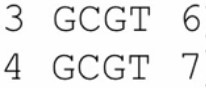
\includegraphics[width=0.25\textwidth,keepaspectratio]{img/alignment/local2}
		\label{img:uniprot}
		%\caption{Tool for pairwise sequence alignment.}
	\end{figure}
\end{block}{}
\end{frame}
%-------------------------------------------------------
%-------------------------------------------------------

%-------------------------------------------------------
%-------------------------------------------------------
\begin{frame}{Global vs Local Alignment}
\begin{figure}[]
	\centering
	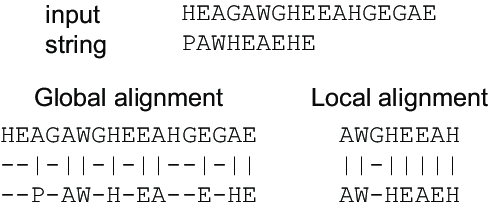
\includegraphics[width=\textwidth,keepaspectratio]{img/alignment/local3}
	\label{img:uniprot}
	%\caption{Tool for pairwise sequence alignment.}
\end{figure}
\end{frame}
%-------------------------------------------------------
%-------------------------------------------------------

%-------------------------------------------------------
%-------------------------------------------------------
\begin{frame}{Global vs Local Alignment}
	Global and local alignment are solve with dynamic programming.
	
	\begin{block}{Global alignment}
		\centering
		Porposed in: \textbf{A general method applicable to the search for similarities in the amino acid sequence of two proteins} by Needleman in 1970 \cite{needleman1970general}.
	\end{block}

	\begin{block}{Local alignment}
		\centering
		Porposed in: \textbf{Identification of common molecular subsequences} by Smith in 1981 \cite{smith1981identification}.
	\end{block}
	
\end{frame}
%-------------------------------------------------------
%-------------------------------------------------------



%%%%%%%%%%%%%%%%%%%%%%%%%%%%%%%%%%%%%%%%%%%%%%%%%%%%%%%%%%%%%%%%%%%%%%%%%%%%%%%%%%%%%%%%%%%%%%%%%%%%%%%%%%%%%%%%
%%%%%%%%%%%%%%%%%%%%%%%%%%%%%%%%%%%%%%%%%%%%%%%%%%%%%%%%%%%%%%%%%%%%%%%%%%%%%%%%%%%%%%%%%%%%%%%%%%%%%%%%%%%%%%%%
\subsection{Local alignment}
%%%%%%%%%%%%%%%%%%%%%%%%%%%%%%%%%%%%%%%%%%%%%%%%%%%%%%%%%%%%%%%%%%%%%%%%%%%%%%%%%%%%%%%%%%%%%%%%%%%%%%%%%%%%%%%%
%%%%%%%%%%%%%%%%%%%%%%%%%%%%%%%%%%%%%%%%%%%%%%%%%%%%%%%%%%%%%%%%%%%%%%%%%%%%%%%%%%%%%%%%%%%%%%%%%%%%%%%%%%%%%%%%


%-------------------------------------------------------
%-------------------------------------------------------
\begin{frame}{Local alignment}{Definition}	
	
	\begin{block}{}
		\justifying
		
		No negative scores are used (use zero instead). A similar tracing-back procedure is used in dynamic programming. However, the alignment path may begin and end internally along the main diagonal. It starts with the highest scoring position and proceeds diagonally up to the left until reaching a cell with a zero \cite{xiong2006essential}.
	\end{block}

\end{frame}
%-------------------------------------------------------
%-------------------------------------------------------

%-------------------------------------------------------
%-------------------------------------------------------
\begin{frame}{Local alignment}{Waterman}	
	\centering	
	\href{https://www.coursera.org/learn/bioinformatics-pku/lecture/eGj3d/interview-with-m-s-waterman-waterman}{\color{blue}{\underline{Interview with Waterman}}}
	\begin{figure}[]
		\centering
		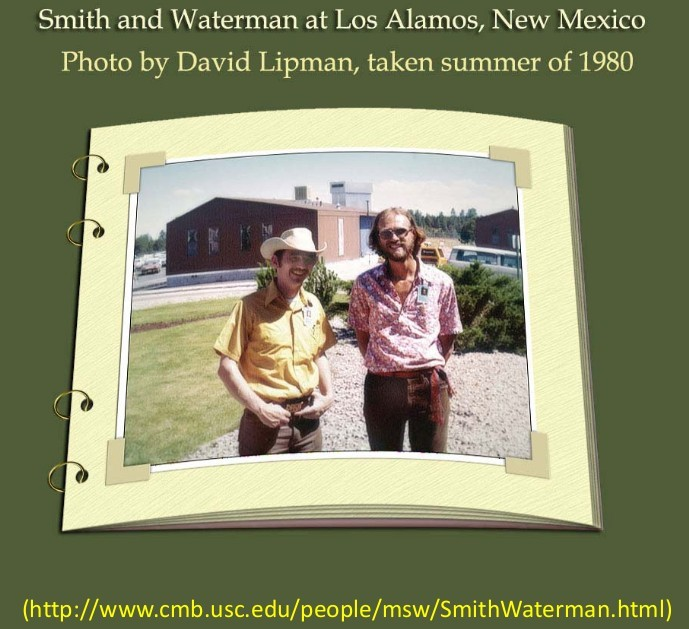
\includegraphics[width=0.7\textwidth,keepaspectratio]{img/alignment/local5}
		\label{img:uniprot}
		%\caption{Alignment: ``|'' stands for equality, ``:'' for similarity and ``.'' for non-similarity.}
	\end{figure}
\end{frame}
%-------------------------------------------------------
%-------------------------------------------------------



%-------------------------------------------------------
%-------------------------------------------------------
\begin{frame}{Local alignment}{Definition}		
	\begin{figure}[]
		\centering
		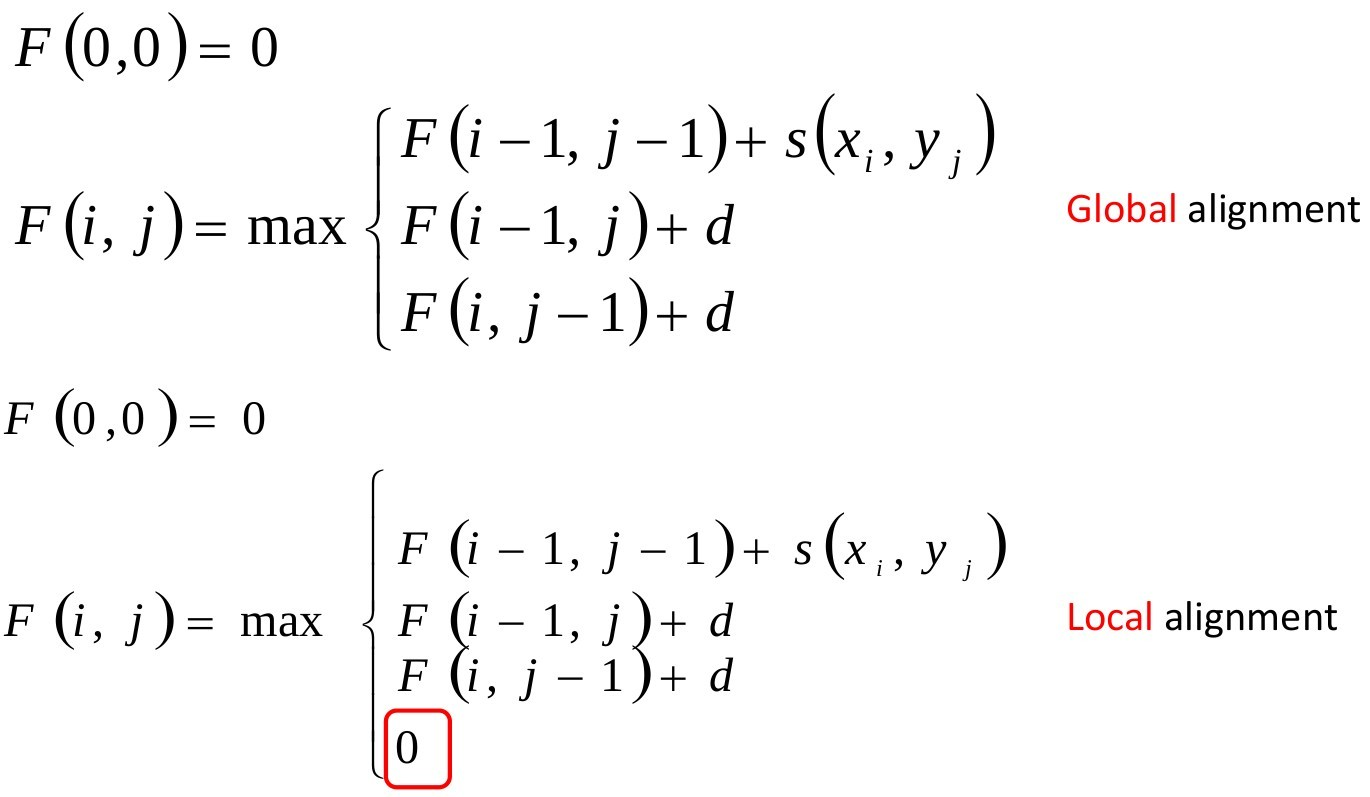
\includegraphics[width=\textwidth,keepaspectratio]{img/alignment/local6}
		\label{img:uniprot}
		%\caption{Alignment: ``|'' stands for equality, ``:'' for similarity and ``.'' for non-similarity.}
	\end{figure}
\end{frame}
%-------------------------------------------------------
%-------------------------------------------------------


%-------------------------------------------------------
%-------------------------------------------------------
\begin{frame}{Local alignment}{Definition}		
	\begin{figure}[]
		\centering
		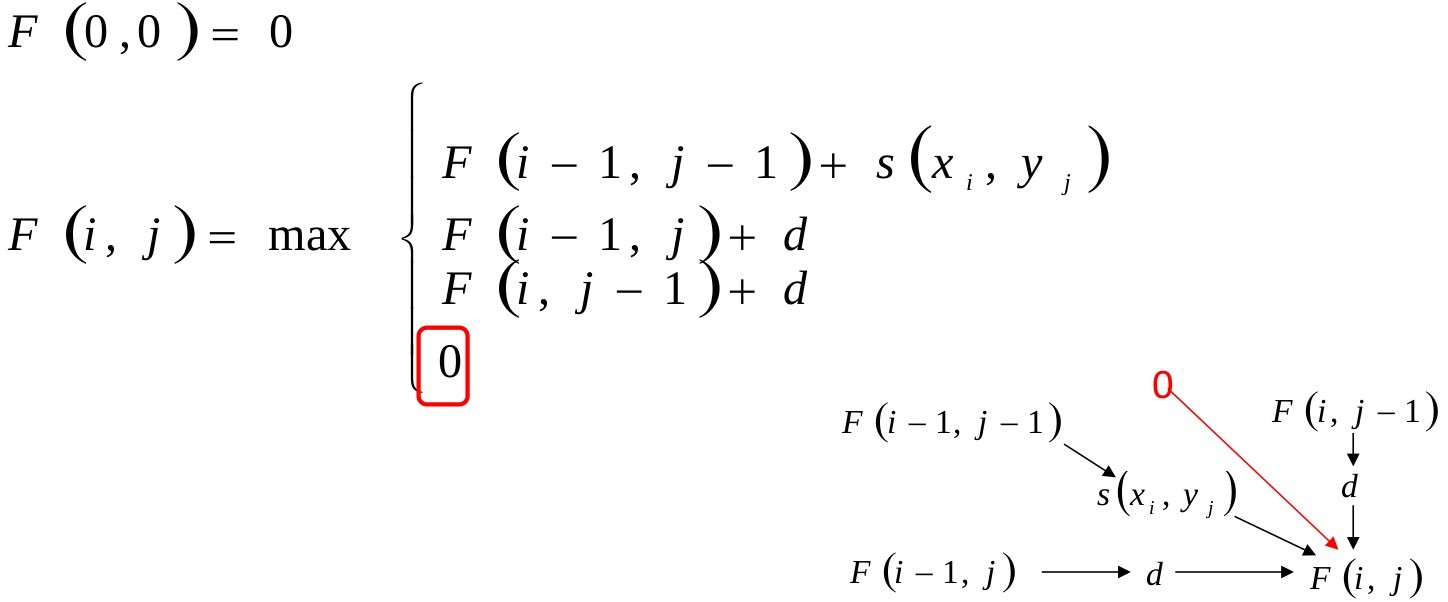
\includegraphics[width=\textwidth,keepaspectratio]{img/alignment/local7}
		\label{img:uniprot}
		%\caption{Alignment: ``|'' stands for equality, ``:'' for similarity and ``.'' for non-similarity.}
	\end{figure}
\end{frame}
%-------------------------------------------------------
%-------------------------------------------------------


%-------------------------------------------------------
%-------------------------------------------------------
\begin{frame}{Local alignment}{Example}		
	\begin{figure}[]
		\centering
		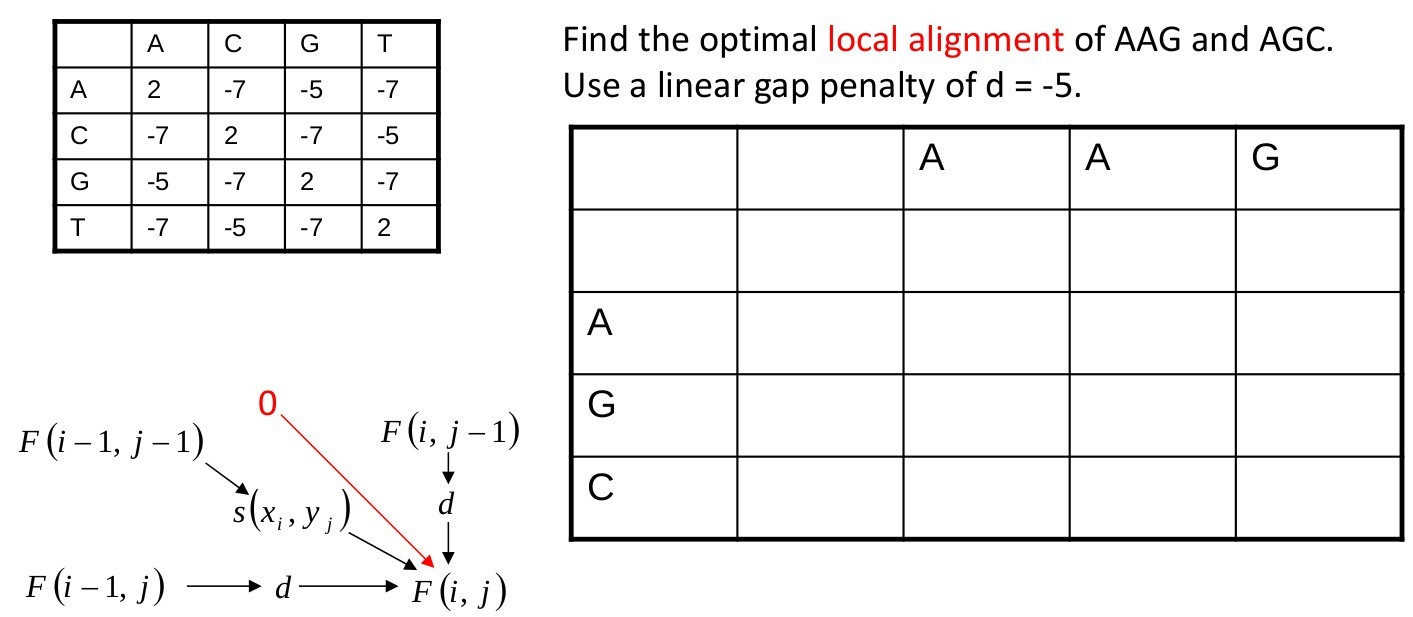
\includegraphics[width=\textwidth,keepaspectratio]{img/alignment/local8}
		\label{img:uniprot}
		%\caption{Alignment: ``|'' stands for equality, ``:'' for similarity and ``.'' for non-similarity.}
	\end{figure}
\end{frame}
%-------------------------------------------------------
%-------------------------------------------------------


%-------------------------------------------------------
%-------------------------------------------------------
\begin{frame}{Local alignment}{Example}		
	\begin{figure}[]
		\centering
		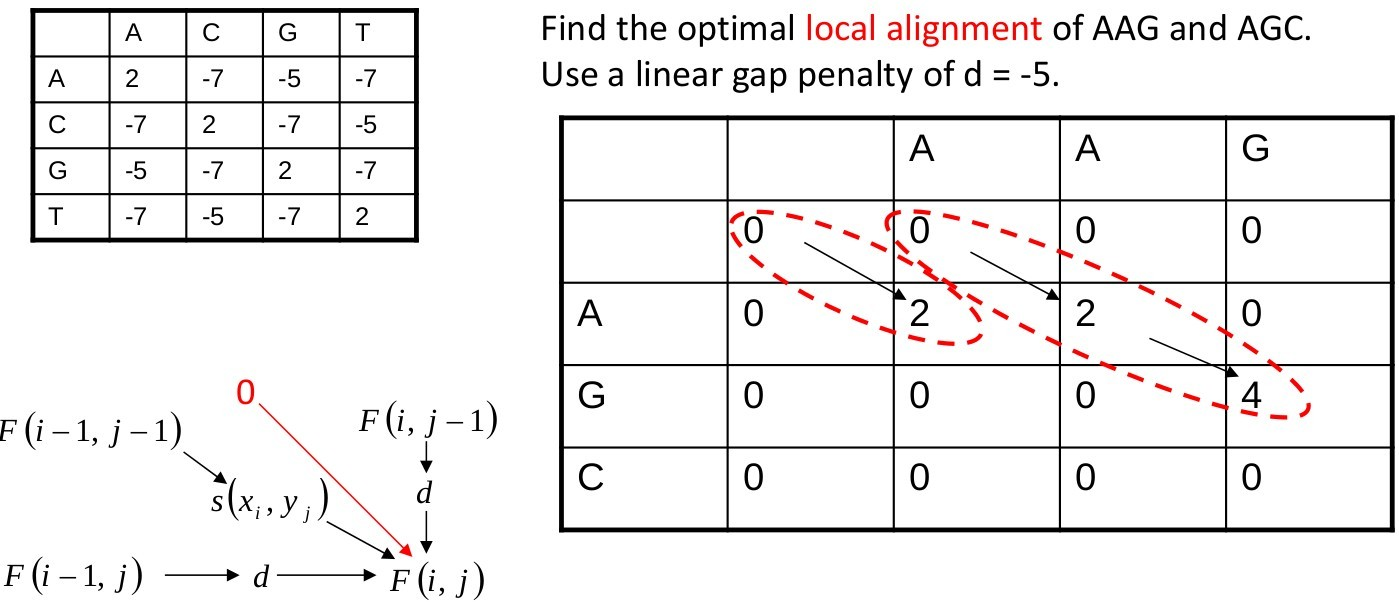
\includegraphics[width=\textwidth,keepaspectratio]{img/alignment/local9}
		\label{img:uniprot}
		%\caption{Alignment: ``|'' stands for equality, ``:'' for similarity and ``.'' for non-similarity.}
	\end{figure}
\end{frame}
%-------------------------------------------------------
%-------------------------------------------------------

%-------------------------------------------------------
%-------------------------------------------------------
\begin{frame}{Local alignment}{Example}	
	Trace back begins at the highest score in	the matrix and continues until you reach 0.
	\begin{figure}[]
		\centering
		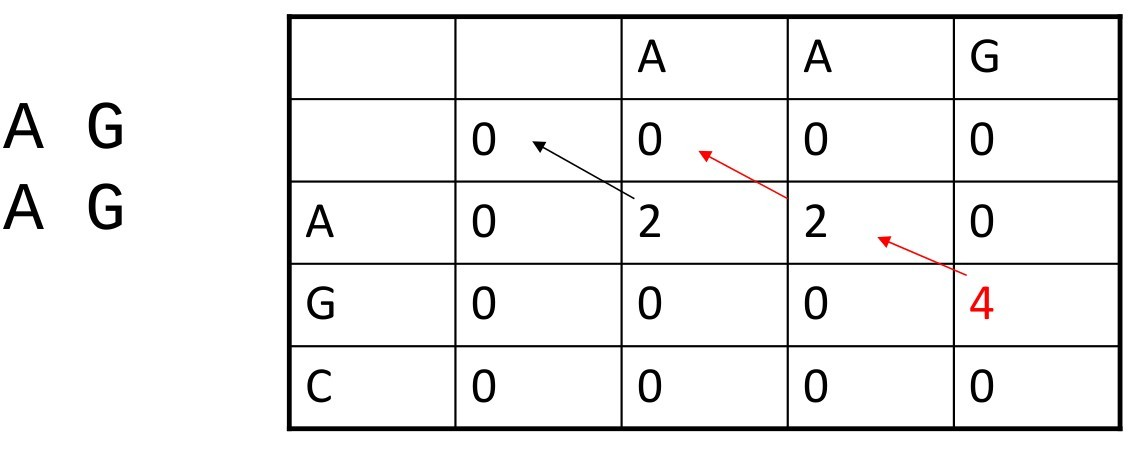
\includegraphics[width=\textwidth,keepaspectratio]{img/alignment/local10}
		\label{img:uniprot}
		%\caption{Alignment: ``|'' stands for equality, ``:'' for similarity and ``.'' for non-similarity.}
	\end{figure}
\end{frame}
%-------------------------------------------------------
%-------------------------------------------------------

%-------------------------------------------------------
%-------------------------------------------------------
\begin{frame}{Local alignment}{Example}	
	And also the secondary best alignment.
	\begin{figure}[]
		\centering
		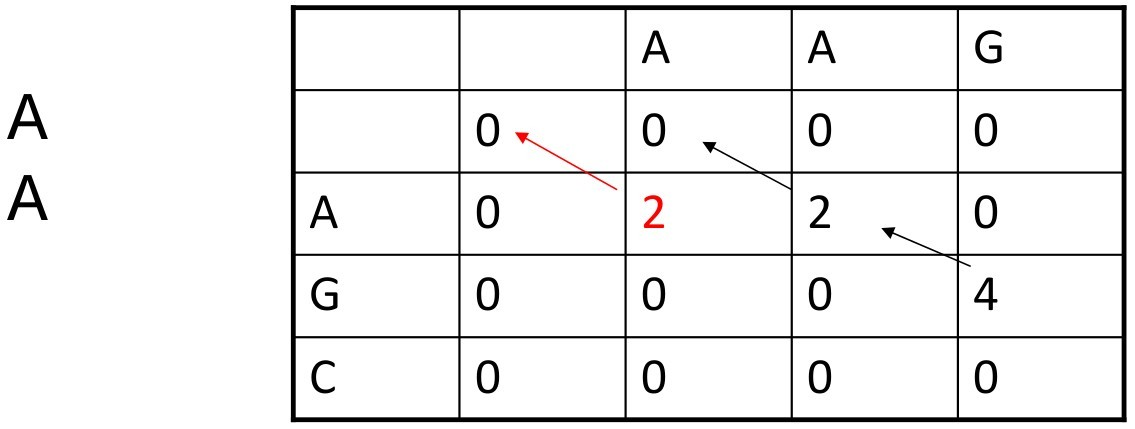
\includegraphics[width=\textwidth,keepaspectratio]{img/alignment/local11}
		\label{img:uniprot}
		%\caption{Alignment: ``|'' stands for equality, ``:'' for similarity and ``.'' for non-similarity.}
	\end{figure}
\end{frame}
%-------------------------------------------------------
%-------------------------------------------------------

%-------------------------------------------------------
%-------------------------------------------------------
\begin{frame}{Local alignment}{Global vs. Local}	

	\begin{figure}[]
		\centering
		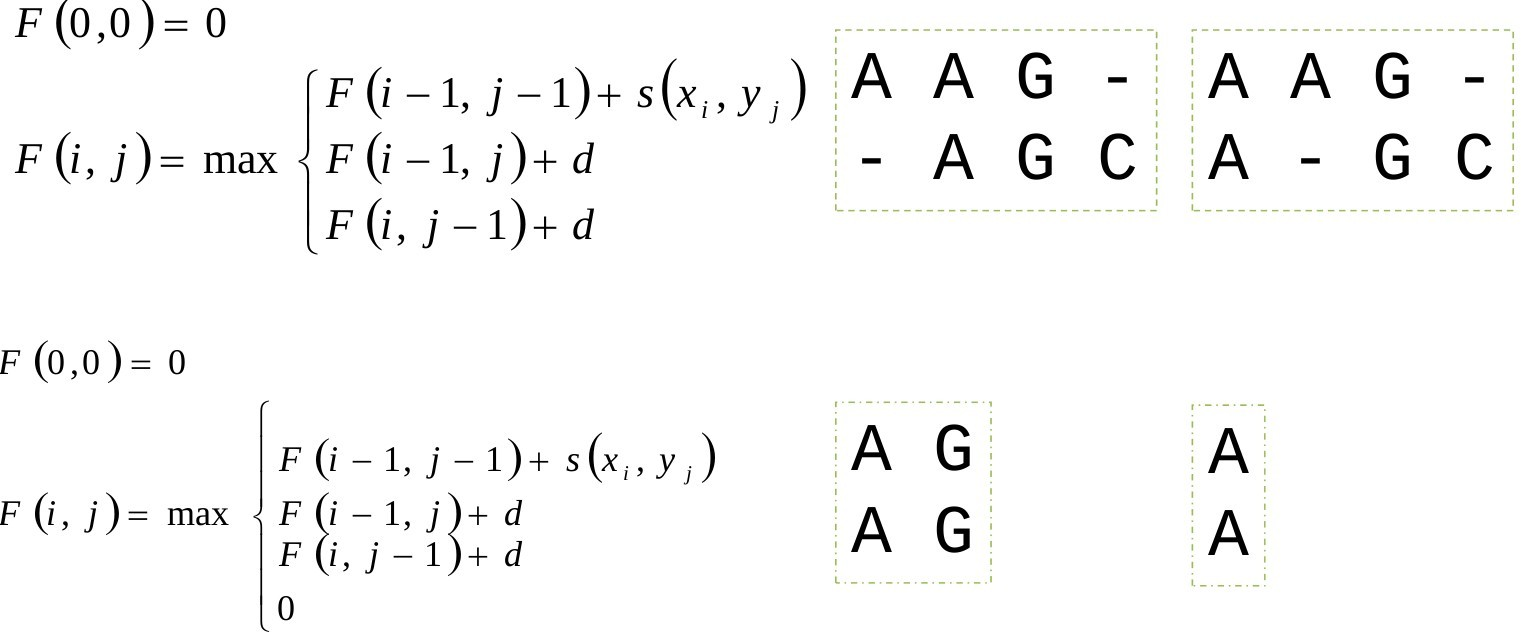
\includegraphics[width=\textwidth,keepaspectratio]{img/alignment/local12}
		\label{img:uniprot}
		%\caption{Alignment: ``|'' stands for equality, ``:'' for similarity and ``.'' for non-similarity.}
	\end{figure}
\end{frame}
%-------------------------------------------------------
%-------------------------------------------------------



%%%%%%%%%%%%%%%%%%%%%%%%%%%%%%%%%%%%%%%%%%%%%%%%%%%%%%%%%%%%%%%%%%%%%%%%%%%%%%%%%%%%%%%%%%%%%%%%%%%%%%%%%%%%%%%%
%%%%%%%%%%%%%%%%%%%%%%%%%%%%%%%%%%%%%%%%%%%%%%%%%%%%%%%%%%%%%%%%%%%%%%%%%%%%%%%%%%%%%%%%%%%%%%%%%%%%%%%%%%%%%%%%
\subsection{Semi Global Alignment}
%%%%%%%%%%%%%%%%%%%%%%%%%%%%%%%%%%%%%%%%%%%%%%%%%%%%%%%%%%%%%%%%%%%%%%%%%%%%%%%%%%%%%%%%%%%%%%%%%%%%%%%%%%%%%%%%
%%%%%%%%%%%%%%%%%%%%%%%%%%%%%%%%%%%%%%%%%%%%%%%%%%%%%%%%%%%%%%%%%%%%%%%%%%%%%%%%%%%%%%%%%%%%%%%%%%%%%%%%%%%%%%%%

%-------------------------------------------------------
%-------------------------------------------------------
\begin{frame}{Semi Global Alignment}{Definition}	
	
	\begin{block}{}
	 In semi global similarity we seek a global alignment where we do not penalize for gaps at one or another end of the string.
	\end{block}

	\begin{block}{}
		The three scores are in general in the following relationship: \\
		\textbf{Global score $\leq$ semi-global score $\leq$ local score}
\end{block}
\end{frame}
%-------------------------------------------------------
%-------------------------------------------------------



%%%%%%%%%%%%%%%%%%%%%%%%%%%%%%%%%%%%%%%%%%%%%%%%%%%%%%%%%%%%%%%%%%%%%%%%%%%%%%%%%%%%%%%%%%%%%%%%%%%%%%%%%%%%%%%%
%%%%%%%%%%%%%%%%%%%%%%%%%%%%%%%%%%%%%%%%%%%%%%%%%%%%%%%%%%%%%%%%%%%%%%%%%%%%%%%%%%%%%%%%%%%%%%%%%%%%%%%%%%%%%%%%
\subsection{Exercises}
%%%%%%%%%%%%%%%%%%%%%%%%%%%%%%%%%%%%%%%%%%%%%%%%%%%%%%%%%%%%%%%%%%%%%%%%%%%%%%%%%%%%%%%%%%%%%%%%%%%%%%%%%%%%%%%%
%%%%%%%%%%%%%%%%%%%%%%%%%%%%%%%%%%%%%%%%%%%%%%%%%%%%%%%%%%%%%%%%%%%%%%%%%%%%%%%%%%%%%%%%%%%%%%%%%%%%%%%%%%%%%%%%

%-------------------------------------------------------
%-------------------------------------------------------
\begin{frame}{Exercises}	
	
	\begin{block}{}
		Local align the following sequences:
		\begin{itemize}
			\item $S_1$ : ACCGTGA
			\item $S_2$ : GTGAATA
		\end{itemize}
		Use this scores: match = +1, mismatch = -1, gap = -1	
	\end{block}
	
	
\end{frame}
%-------------------------------------------------------
%-------------------------------------------------------

%-------------------------------------------------------
%-------------------------------------------------------
\if\mycmd1 % MY THEME
\1{
	{\1
		\begin{frame}[plain,noframenumbering]
			%\finalpage{Thank you}
			\begin{figure}[]
				\centering
				
\includegraphics[width=\textwidth,height=0.7\textheight,keepaspectratio]{img/question.png}
				%\label{img:mot2}
				%\caption{Image example in 2 gray levels.}
			\end{figure}
	\end{frame}}
	\else % CS THEME
	\begin{frame}{Questions?}
		\begin{figure}[]
			\centering
			
\includegraphics[width=\textwidth,height=0.7\textheight,keepaspectratio]{img/question.png}
			%\label{img:mot2}
			%\caption{Image example in 2 gray levels.}
		\end{figure}
		
	\end{frame}
	\fi
	%-------------------------------------------------------
	%-------------------------------------------------------

%-------------------------------------------------------
%-------------------------------------------------------
\begin{frame}[allowframebreaks]
	\frametitle{References}
	%\bibliographystyle{amsalpha}
	\bibliographystyle{IEEEtran}
	\bibliography{bibliography.bib}
\end{frame}
%-------------------------------------------------------
%-------------------------------------------------------

\end{document}